%*****************************************************************************************
%*********************************** First Chapter ***************************************
%*****************************************************************************************

\chapter{Introduction}

\graphicspath{{Chapter1/Figures/}}

Semiconducting behaviour was first reported by Michael Faraday, who noted in 1839 that the conductivity of silver selenide increased with temperature, opposite to what was expected for metals \cite{Faraday2012}. Photovoltaic behaviour was observed in silver chloride coated platinum electrodes, where illumination with sunlight caused an increase in the induced voltage \cite{Becquerel1839}, while the first photovoltaic cell used 30\,$\mu$m thick selenium film and was <1\% efficient \cite{Fritts1883}. Photoconductivity was shown by selenium as a result of exposure to sunlight \cite{Smith1873, Adams1876}, while electroluminescent behaviour was first seen in silicon carbide \cite{Round1907}. Simple principles such as these underpin the electronic devices we use today, yet it was not until Alan Wilson's work on band theory in 1931 that semiconductor behaviour could be understood and explained \cite{Wilson1931}. 

Throughout the 20th century research was focused on using semiconductors for devices, from the development of rectifiers and diodes in the early part of the century to the first germanium transistor built at Bell Laboratories in 1946 [Fig.\,\ref{1Fig1}(a)]. Since then, much work has been undertaken to refine and improve these designs, however device efficiency still hinges on the quality of the semiconducting materials used, as well as the ability to control impurities and dopants. While the earliest devices used materials such as lead selenide, silicon and germanium are now commonly used.

Silicon is most widely used in the semiconductor industry due to its abundance in the Earth's crust, low unit cost and well-developed processing techniques. A high band gap (1.11\,eV at 300\,K \cite{Kittel1986}) gives it thermal stability, allowing silicon to be used at high operating temperatures. In addition, silicon is highly mechanically stable with high electron mobility, and the native insulating oxide layer can be useful in electronics. Although germanium has higher conductivity, a lower band gap (0.66\,eV at 300\,K \cite{Kittel1986}) leads to more temperature sensitive devices, although alloys of silicon and germanium may be used to combine the properties of both materials. However both materials have indirect band gaps and thus poor emission properties, so alloys of Group III-V or II-VI elements are typically used in luminescent devices. The properties of such alloys can be tuned via composition to produce the optoelectronic characteristics required, alternatively lower dimension structures can be created to provide other desirable attributes. For example, gallium arsenide has a large direct band gap (1.43\,eV at 300\,K \cite{Kittel1986}) and high electron mobility, which means it is suitable for high speed devices.
\begin{figure}[h!]
\centering
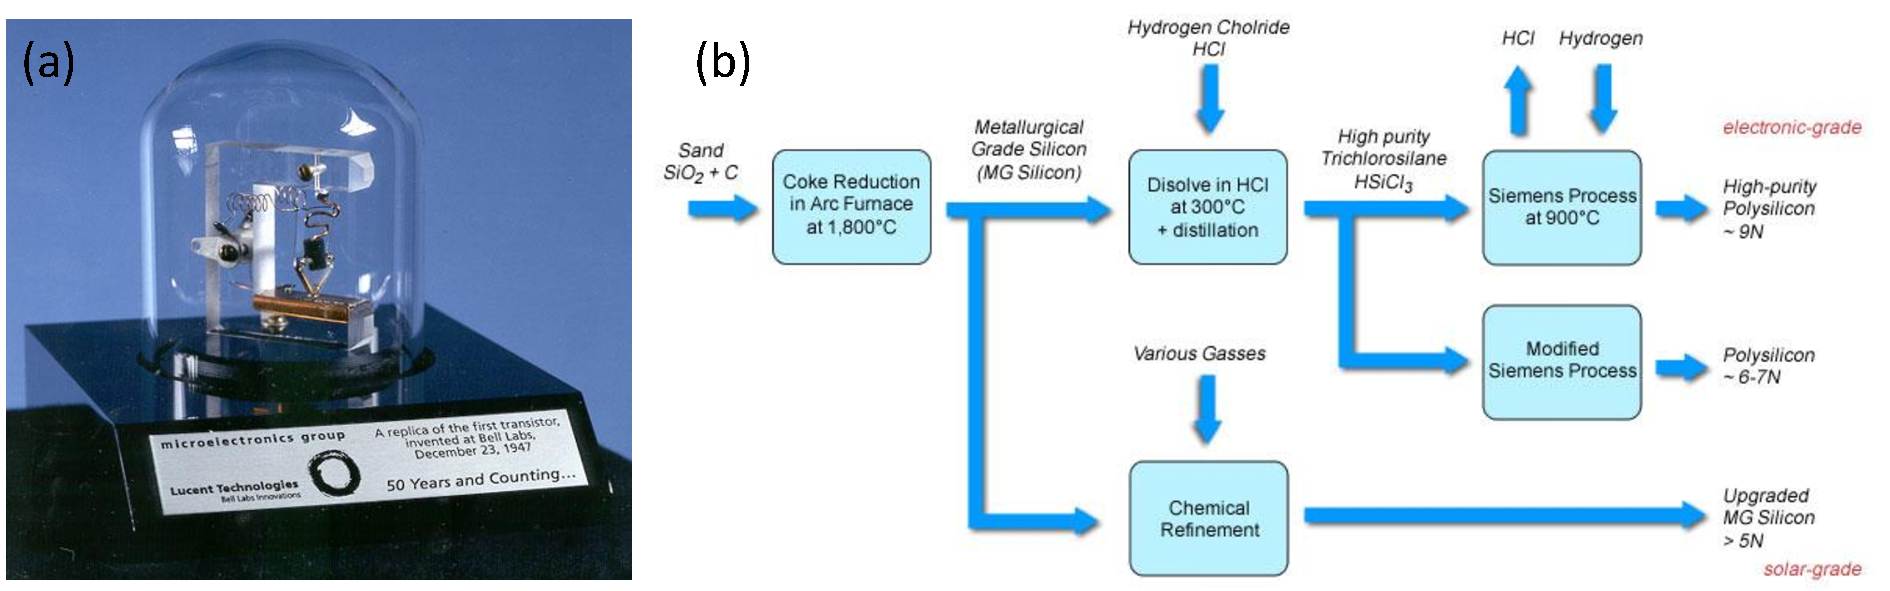
\includegraphics[width=\textwidth]{Fig1}
\caption{(a) Replica of first transistor built in 1946. Reproduced from Ref.\,\cite{Transistor}. (b) Process required to produce device-grade silicon from starting materials \cite{Silicon}.}
\label{1Fig1}
\end{figure}

Despite the high stability and carrier mobility shown by inorganic semiconductors, one major disadvantage is with the processing of such materials. Although silicon processing is well-developed, creation of device-grade material still requires many purification steps [Fig.\,\ref{1Fig1}(b)]. Alloys are often produced using vapour or electron-beam deposition, where deposition parameters must be strictly controlled. Layer-by-layer growth can be used for the best quality samples, however such processes are costly and time consuming. Current advances in technology require flexible, lightweight and more easily processable semiconductors, as well as control over the behaviour of carriers, for example the formation of new quasiparticles via strong coupling.

\begin{figure}[h!]
\centering
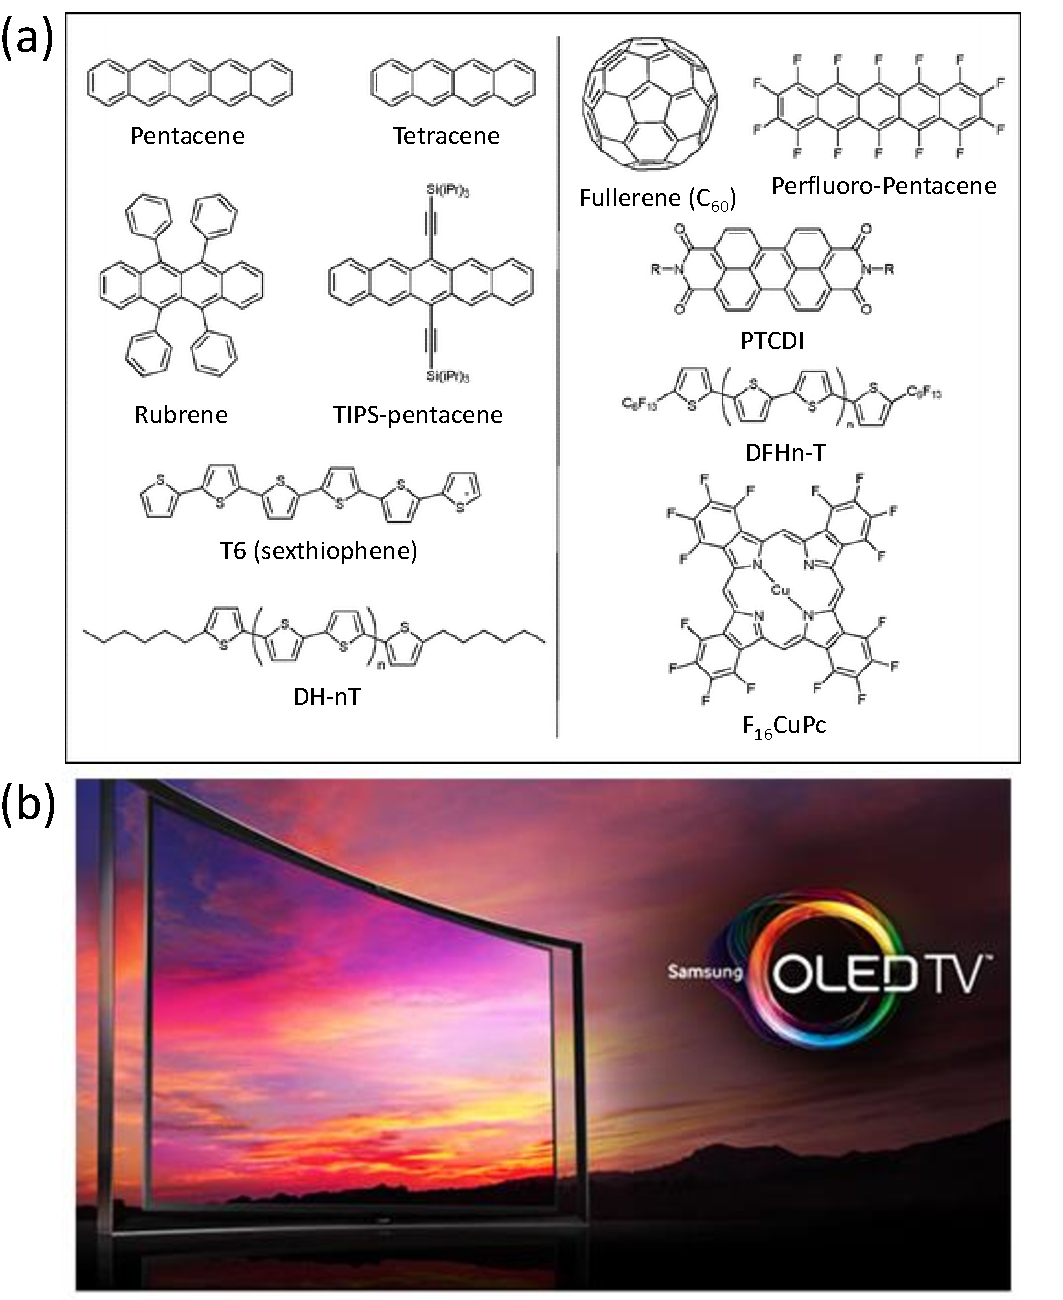
\includegraphics[width=0.8\textwidth]{Fig2}
\caption{(a) Common organic semiconductors. P-type materials on shown the left, and n-type on the right. Modified from Ref.\,\cite{Miozzo2010}. (b) Samsung curved smart OLED TV. Reproduced from Ref.\,\cite{Samsung}.}
\label{1Fig2}
\end{figure}
Although conduction was noted in a mix of aniline and sulphuric acid by Henry Letherby in 1862, research on organic semiconductors began in earnest in the latter half of the 20th Century. Polycyclic aromatic compounds were found to form semiconducting charge transfer complexes with halogens \cite{Naarmann2002}, and since then much work has been done on developing new molecules and polymers, driven by the relative ease with which such molecules can be synthesised. Organic semiconductors generally consist of conjugated molecules, whose overlapping $\pi$ orbitals allow charge transport within the molecule [Fig.\,\ref{1Fig2}(a)]. Given the low production cost, work has been undertaken to produce devices made of organic semiconductors, notably photovoltaics, thin film transistors, and organic light emitting diodes (OLEDs). OLEDs are the most technologically mature application of organic electronics as they are currently used mobile phone displays and TVs, and offer better efficiency and brightness than other display technologies [Fig.\,\ref{1Fig2}(b)]. However problems exist with the manufacture of such devices as mass production is not currently optimised for the organic electronic market. More fundamentally, organic semiconductors are less thermally, optically and electrically stable than their inorganic counterparts, leading to lower device lifespan. Charge mobility is also lower as hopping between adjacent molecules is required, and lower crystallinity leads to increased scattering at grain boundaries. 

A new class of hybrid materials has emerged in the last 25 years. Metal halide-based organic-inorganic perovskite semiconductors combine the stability of the inorganic semiconductors with the processability of organic semiconductors. A variety of self-assembling of inorganic frameworks can form and accommodate excited charge carriers, while organic moieties can be used to further modify material properties \cite{Cheng2010, Ishihara1990, Mitzi2001, Mitzi2001c, Nagami1996, Pradeesh2010, Pradeesh2009a, Lee2012, Heo2013, Liu2013, Hao2014}. Such perovskites can be incorporated into nanostructures to form new mixed states with novel optoelectronic properties \cite{Fujita1998, Fujita1999, Fujita2000, Ishi-Hayase2003, Brehier2006, Lanty2008, Pradeesh2009b, Sumioka2001}.

This thesis explores the optical properties of 2D lead iodide-based perovskites, particularly the interactions between perovskite excitons and collective electron oscillations called surface plasmons. In Chapter 2 I will introduce the theory of excitons and review the research on lead iodide perovskites, before exploring the optical properties of noble metal nanostructures in Chapter 3. Chapter 4 describes the fabrication of spin-coated perovskite thin films, and investigates how changes in film morphology affect optical spectra. Chapter 5 examines the optical properties of ultra-thin perovskite samples produced via exfoliation, using spectra to infer nanoscale structural changes. In the next two Chapters hybrid semiconductor-metal nanostructures are used to illustrate the effect electrons have on excitons: firstly interactions between excitons and localised surface plasmons in perovskite-coated metallic nano-islands in Chapter 6, then coupling between excitons and surface plasmon polaritons in perovskite-coated plasmonic gratings. Finally the thesis concludes in Chapter 8 with an outlook on future lines of investigation.